\documentclass{report}
\usepackage{parskip}
\usepackage{xcolor}
\usepackage{pgf}
\usepackage{tikz}
\usepackage{hyperref}
\usepackage{natbib}
\usepackage{amssymb}
\usepackage{amsmath}
\usetikzlibrary{decorations.text}
\newcommand*{\mytextstyle}{\sffamily\Large\bfseries\color{black!85}}
\newcommand{\arcarrow}[8]{%
% inner radius, middle radius, outer radius, start angle,
% end angle, tip protusion angle, options, text
  \pgfmathsetmacro{\rin}{#1}
  \pgfmathsetmacro{\rmid}{#2}
  \pgfmathsetmacro{\rout}{#3}
  \pgfmathsetmacro{\astart}{#4}
  \pgfmathsetmacro{\aend}{#5}
  \pgfmathsetmacro{\atip}{#6}
  \fill[#7] (\astart:\rin) arc (\astart:\aend:\rin)
       -- (\aend+\atip:\rmid) -- (\aend:\rout) arc (\aend:\astart:\rout)
       -- (\astart+\atip:\rmid) -- cycle;
  \path[font = \sffamily, decoration = {text along path, text = {|\mytextstyle|#8},
    text align = {align = center}, raise = -0.5ex}, decorate]
    (\astart+\atip:\rmid) arc (\astart+\atip:\aend+\atip:\rmid);
}
\bibliographystyle{unsrtnat}
\usetikzlibrary{arrows,automata}
\title{Final IT Report}
\author{Vivian Ye-Ting Dang (\texttt{z5118468})}
\setlength{\parindent}{0pt}
\newcommand{\TODO}[1]{\textcolor{red}{#1}}
\begin{document}
\maketitle
\tableofcontents

\chapter*{Abstract}
This report contains details relating to the compulsory industrial training 
that I have carried out as required for the Engineering degree at the University of New South Wales.
It is written in the format provided by the UNSW Engineering Industrial Training Guideline.
I have completed a total of 60 days (12 weeks) of industrial training over one full-time placement.

\chapter{Introduction}
I completed my industrial training internship with the programming languages (PL) and formal methods 
(FM) team at Cog Systems Pty Ltd in Sydney. 
Cog Systems leads the industry in secure connected device implementations across world governments, 
defense organizations and corporate enterprises.
They have adopted an embedded solution built on modularity, proactive security, trustworthiness, 
and adaptability to enable highly secure connected devices.

The PL and FM team at Cog Systems makes use of the latest academic research as well as 
industry practices to enable IoT components to be provably free of software bugs and of security 
vulnerabilities.

I worked with Kai Engelhardt, a senior principal engineer at Cog and also the leader of the PL and 
FM team. 
As a software engineering intern, I was given a wide variety of tasks and responsibilities to 
ensure that I have as much exposure to real world industry practice as possible.
Some of these tasks included designing, building and testing backends of a domain specific 
language (DSL) compiler, a library for inter-process communication (IPC) 
as well as the implementation of an input/output primitive for the language.
These tasks required predominantly programming, debugging and testing as well as frequent 
discussions with my project lead and extensive research from academic sources and documentation.

I worked full-time between the 19th of November 2018 and 15th February 2019 (with a week worth of 
leave in between) for a total of 60 days.

\chapter{Engineers Australia Competencies}
\section{Knowledge and Skill Base}
\textit{(1.2) Conceptual understanding of the mathematics, numerical analysis, statistics, and
computer and information sciences which underpin the engineering discipline}

I was given the opportunity to work on developing a DSL that describes a concurrent system based on
message-passing IPC. These systems are typically described in the literature using Kripke 
structures~\citep{kripke}
and reasoned about using Linear Temporal Logic (LTL)~\citep{Pnueli}. An example of such a system is 
given in \autoref{fig:kripke}.
There are two processes, one representing a traffic light and the other representing a vehicle.
The vehicle is only able to drive while the light is green. This property can be expressed in LTL as
$$\square (\text{Drive}\Rightarrow \text{Green})$$

\begin{figure}
    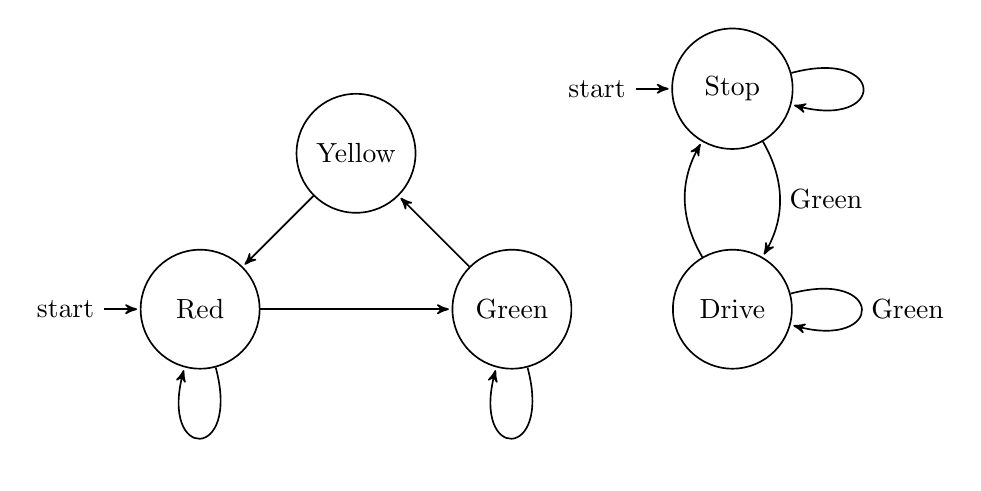
\begin{tikzpicture}[->,>=stealth',shorten >=1pt,auto,node distance=2.8cm,
        semithick]
        \tikzstyle{every state}=[text width=1.2cm, align=center]

        \node[initial,state] (R)              {Red};
        \node[state]         (Y) [above right of=R] {Yellow};
        \node[state]         (G) [below right of=Y] {Green};

        \path (R) edge (G)
        edge [loop below] (R)
        (G) edge (Y)
        (G) edge [loop below] (G)
        (Y) edge (R);

        \node[state]         (D) [right of=G] {Drive};
        \node[initial,state] (S) [above of=D] {Stop};
        \path (S) edge [bend left] node {Green} (D)
        (S) edge [loop right] (S)
        (D) edge [loop right] node {Green} (D)
        (D) edge [bend left] (S);
    \end{tikzpicture}
\caption{An example of a Kripke Structure that models a traffic light}
\label{fig:kripke}
\end{figure}
PROMELA (Process or Protocol Meta Language) is a verification modelling language that allows the
modelling of concurrent processes. The process can then be visualised and automatically verified
using Spin, which is a tool to conduct logical verification of concurrent software.  
I developed part of the compiler of the DSL that translated from the DSL to PROMELA. 

I undertook a relevant course at UNSW, Concepts of Programming Languages (COMP3161), which taught me 
useful skills that I could apply in the development of a programming language. This involves being
able to work with a parser and typechecker, which is what I was required to do in the DSL compiler
in order to translate from the DSL to PROMELA.

In addition, I also developed a message-passing IPC library to allow the users to simulate their DSL
programs based on the concept of channels similar to \citet{Hoare}. For this, I used the Portable 
Operating System Interface (POSIX) standardised library \texttt{pthreads}~\citep{mueller}.

\textit{(1.4) Discernment of knowledge development and research direction within the engineering
discipline}

Over the last decade, formal methods aimed at complete, end-to-end verification of software 
systems have become more popular, with many successes including verified compilers for 
C~\citep{compcert} and ML~\citep{cakeml}, verified theorem provers Milawa~\citep{milawa} and 
Candle~\citep{candle}, a verified conference system~\citep{cocon}, a crash-resistant 
file system~\citep{fscq}, the concurrency verification in CertiKOS~\citep{certikos}, 
the verified cryptographic routines of OpenSSL HMAC~\citep{openssl}, the verified distributed 
system Ironfleet~\citep{ironfleet} and many more.

The aforementioned IPC library was intended to facilitate the compilation of the DSL to the 
new research language Cogent. Cogent is a recent research language aimed at reducing the cost 
of end-to-end formal verification of systems~\citep{asplos}. This opens up a new frontier for 
verified systems, by allowing users to easily prove once and for all that their software meets requirements
in the form of a correctness specification. This proof also integrates with the world-famous 
verified seL4 microkernel~\citep{sel4}, itself a game-changer in the world of high-assurance systems software.

Cogent is a purely functional language based on uniqueness types~\citep{liam}. This type system 
allows specifications written in a mathematical style to be compiled to efficient C implementations~\citep{wadler}.
Cog envisions connecting their DSL up to the Cogent language, thus enabling their software to be 
formally verified to be free of correctness bugs.


\textit{(2.2) Fluent application of engineering techniques, tools, and resources.}

My role involved a lot of programming, specifically in \citet{haskell}, which is a functional programming
language that is seeing increasing use in high-assurance softare development. Partly for this reason,
Cog decided to use Haskell for the DSL development. I completed the course 
Software System Design and Implementation (COMP3141) at UNSW which equipped me with Haskell proficiency
as well as best practice in high-assurance software engineering.

As mentioned in the previous section, I also learnt PROMELA and how to use SPIN during my placement
in order to be able to implement the part of the compiler that translates the DSL into PROMELA.
I achieved this mainly through reading documentation and asking for help from my direct supervisor
at work when I got stuck. This is notably different from the learning environment at UNSW, where 
skills are imparted directly by teaching staff. I had to get used to considerable self-directed learning,
a point I will expand upon in Chapter~\ref{ch:reflection}.

Another tool I used is Git, which is a common collaboration tool in the industry, used to track multiple versions of 
software source code and their authorship, allowing multiple users to collaborate on the same code 
base and to isolate when bugs are introduced in the development process.
While I was exposed to this tool in many courses that I have completed
throughout my degree at UNSW, this is one of the first times I used it in a large-scale professional context.

\textit{(2.4) Application of systematic approaches to the conduct and management of engineering
projects}

Our project followed the Agile method~\citep{agile}, which involves repeating the Software 
Development Life Cycle (SDLC); a summary of the cycle is shown in \autoref{fig:sdlc}. 

The cycle starts with requirements analysis, this includes identifying the 
problem statement with my supervisor and other members of the company and come up with specification
that contains the acceptance criteria for all the features that have to be completed in the tasks
assigned to me.

The next stage is design, which means evaluating different approaches to solving the problem and
weighing the pros and cons for each approach to decide which one seems best for fulfilling the
requirements, also taking time and resources into consideration.

Then I move on to the development phase, where I implement a minimal viable product (MVP)
that satisfies the previously stated acceptance criteria. This is a minimal implementation 
that \emph{only} satisfies the acceptance criteria, and is intentionally kept small to aid maintainability 
and flexibility for future changes.

After this, the product undergoes testing. This testing is based on the acceptance criteria,
as well as other internal engineering concerns, such as maintanability and performance.
Based on the information gained through testing, as well as feedback from stakeholders,
changes are made to the specification, and faults are isolated and fixed. Once the appropriate
specification changes have been made, the cycle repeats again, this time focusing on the implementation
of new features or other requested changes.

\begin{figure}
    \centering
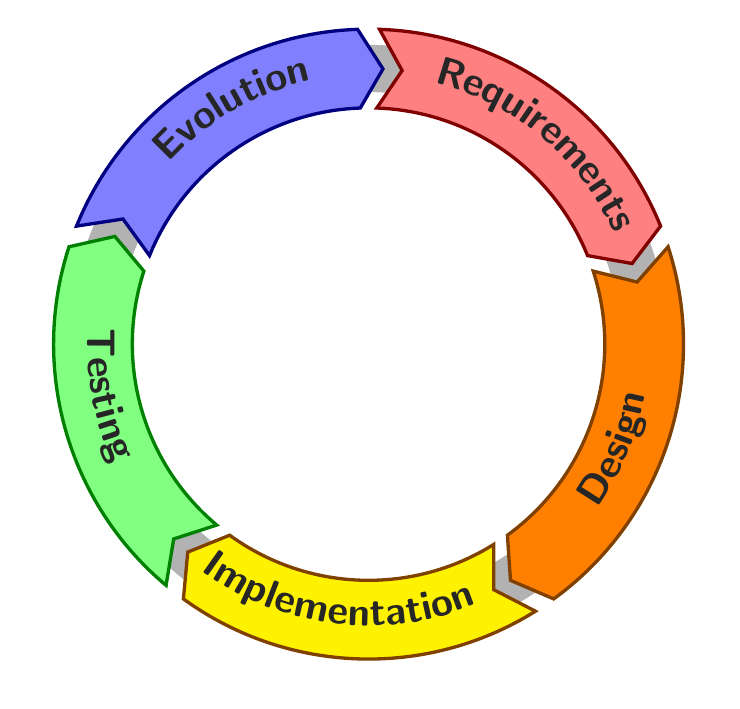
\begin{tikzpicture}
    \fill[even odd rule,black!30] circle (3.8) circle (3.2);
      \arcarrow{3}{3.5}{4}{88}{22}{-5}{red!50!white,
        draw = red!50!black, very thick}{Requirements};
      \arcarrow{3}{3.5}{4}{-54}{18}{-5}{orange,
        draw = orange!50!black, very thick}{Design};
      \arcarrow{3}{3.5}{4}{-126}{-58}{-5}{yellow,
        draw = orange!50!black, very thick}{Implementation};
      \arcarrow{3}{3.5}{4}{-198}{-130}{-5}{green!50!white,
        draw = green!50!black, very thick}{Testing};
      \arcarrow{3}{3.5}{4}{-202}{-268}{-5}{blue!50!white,
        draw = blue!50!black, very thick}{Evolution};
  \end{tikzpicture}
\caption{The Software Development Life Cycle (SDLC)}
\label{fig:sdlc}
\end{figure}

\textit{(3.5) Orderly management of self, and professional conduct}

While this report may seem to indicate that I was given a number of concrete tasks to achieve 
during my placement, the tasks I completed were mostly the result of collaborative research 
efforts with the rest of my team. 

This meant that it was crucial for me to concretize and reify the requirements placed on my 
team into specific tasks that could be completed with precise evaluation and acceptance criteria.

As this project had a considerable focus on new research, it was vital that I maintained my connections
with UNSW research staff, with whom Cog collaborated for this project. This also enabled me to 
further my own studies in this discipline, and explore new avenues for future research that I 
am carrying out in my undergraduate thesis.

This was a fortunate confluence of ambitions, as I wished to improve my knowledge in the 
formal methods and programming languages spaces, Cog wished to improve their products using 
this knowledge, and my UNSW friends and colleagues were able to assist both me personally and Cog 
professionally in this context.

In order to ensure that my tasks were completed in a timely manner, I broke down my tasks 
into small, achievable components with self-set deadlines. This deadline pressure is an effective way
to ensure that I do not let myself become distracted by interesting research problems that do not 
align with organisational objectives.

\chapter{Reflection \& Conclusion}
\label{ch:reflection}

My experience in this industrial placement brought into stark relief several interesting distinctions
between learning in an academic context and through an internship position. 

One of the main aspects of the industry that I noticed is the emphasis on self-directed learning 
and development. In a university course, I could reasonably expect to find all the information 
necessary for understanding a particular topic to be available from the provided course materials. 
By contrast, the industrial setting poses much more open-ended problems where the solutions 
are not necessarily known, even by more senior members of staff. Therefore, I had to undertake 
significant study projects independently in order to gain the skills necessary to achieve the 
milestones set for me. If I needed assistance, I would have to take initiative to seek it out myself, 
rather than rely on my supervisors or other superiors to provide me with information.

While this is significantly different from most UNSW coursework, it is not that dissimilar to 
the undergraduate thesis project I am now undertaking. This project, being a research thesis, 
also involves a number of open-ended problems, and independent, self-directed study. 

Another aspect of industry that I observed is that team-work is the default. Individual, independent
projects are exceptionally rare in the software industry, as opposed to a university setting, where,
despite some group-work projects, the majority of work is necessarily conducted individually.
Because of this, it is necessary to forge social relationships with colleagues in an industry environment,
whereas in university, such relationships are strictly an extra-curricular activity.

The structure of an industry workplace is also markedly different from that of university. For example,
an eight-hour work day took considerable getting used to, coming from the sporadic class timetables 
of university life. Also, the physical work environment differs too, as I was given a fixed desk in 
an open-plan office, whereas at UNSW, work is conducted wherever I can find a place to sit.\footnote{Also, this is becoming increasingly difficult.}

I also was able to significantly expand my technical knowledge during this placement, which has in
turn assisted me in my coursework and undergraduate thesis. Seeing as my thesis also involves the 
Cogent language, and Programming Languages more generally, much of what I learned at Cog applies 
directly to my current studies.

Overall, I feel that this placement was immensely valuable to me. It helped me to develop my 
professional communication skills, widen my technical knowledge, and forge new personal relationships.

\bibliography{cites}

\chapter{Appendix}

\end{document}